\documentclass[conference]{IEEEtran}
\IEEEoverridecommandlockouts
% The preceding line is only needed to identify funding in the first footnote. If that is unneeded, please comment it out.
\usepackage{cite}
\usepackage{amsmath,amssymb,amsfonts}
\usepackage{algorithmic}
\usepackage{graphicx}
\usepackage{textcomp}
\usepackage{xcolor}
\usepackage{fancyhdr}
\usepackage{graphicx}
\usepackage{tabularx}
\usepackage{ragged2e}
\usepackage{makecell}

\def\BibTeX{{\rm B\kern-.05em{\sc i\kern-.025em b}\kern-.08em
		T\kern-.1667em\lower.7ex\hbox{E}\kern-.125emX}}

\fancypagestyle{firstpagestyle}{
    \fancyhf{}
    \renewcommand{\headrulewidth}{0pt}
    \fancyfoot[L]{ 
    $^1$mengikat data antara \textit{model} dan \textit{view} yang disinkronkan setiap terjadinya perubahan
    }
}

\fancypagestyle{secondpagestyle}{
    \fancyhf{}
    \renewcommand{\headrulewidth}{0pt}
    \fancyfoot[L]{ 
    $^2$kode yang digunakan berulang-ulang tanpa perubahan yang signifikan 
    
    $^3$beban tambahan dalam proses komunikasi atau eksekusi
    }
}

\bibliographystyle{unsrt}
    
\begin{document}
	
	\title{Perbandingan Performa Pola Arsitektur \textit{Model-View-Presenter} (MVP) dengan \textit{Model-View-ViewModel} (MVVM)\\
	}
	
	\author{\IEEEauthorblockN{Allycia Joan Micheline}
		\IEEEauthorblockA{\textit{Informatika} \\
			\textit{Universitas Pradita}\\
			Tangerang, Indonesia \\
			allycia.joan@student.pradita.ac.id}
		\and
		\IEEEauthorblockN{Bryant Nehemia Natanael}
		\IEEEauthorblockA{\textit{Informatika} \\
			\textit{Universitas Pradita}\\
			Tangerang, Indonesia \\
			bryant.nehemia@student.pradita.ac.id}
		\and
		\IEEEauthorblockN{Sibgah Rabbani Kusuma}
		\IEEEauthorblockA{\textit{Informatika} \\
			\textit{Universitas Pradita}\\
			Tangerang, Indonesia \\
			sibgah.rabbani@student.pradita.ac.id}
		\and
		\IEEEauthorblockN{Noven Austin}
		\IEEEauthorblockA{\textit{Informatika} \\
			\textit{Universitas Pradita}\\
			Tangerang, Indonesia \\
			noven.austin@student.pradita.ac.id}
	}
	
	\maketitle
	
	\begin{abstract}
		Penelitian ini membandingkan performa kecepatan dan penggunaan memori antara Model-View-Presenter (MVP) dan Model-View-ViewModel (MVVM) dalam pengembangan aplikasi Android. Melalui studi literatur, MVP memiliki penggunaan memori yang lebih efisien, sedangkan MVVM memiliki penggunaan CPU lebih efisien dan waktu eksekusi yang lebih cepat. Setelah melakukan pengujian, MVP unggul dalam penggunaan memori, sementara waktu eksekusi MVVM lebih cepat. Secara keseluruhan, pemilihan antara pola arsitektur MVM dan MVVM harus mempertimbangkan kebutuhan proyek dan karakteristik masing-masing pola arsitektur.
	\end{abstract}
	
	\begin{IEEEkeywords}
		MVP, MVVM, Android
	\end{IEEEkeywords}
	
	\section{Pendahuluan}
	Dalam dunia pengembangan perangkat lunak, pemilihan pola arsitektur sangatlah penting untuk memastikan keberhasilan proyek dan kualitas aplikasi yang dihasilkan. Dua pola arsitektur yang sering digunakan pengembangan aplikasi berbasis Android adalah \textit{Model-View-Presenter} (MVP) dan \textit{Model-View-ViewModel} (MVVM). 
 
    MVP dan MVVM memisahkan aplikasi menjadi tiga komponen utama, yaitu \textit{Model} (menyimpan data dan logika bisnis), \textit{View} (menampilkan antarmuka pengguna), dan \textit{Presenter} (menghubungkan \textit{Model} dan \textit{View} serta mengatur logika pengontrol) untuk MVP \cite{Dan2020}, sedangkan MVVM tidak menggunakan \textit{Presenter} namun \textit{ViewModel} yang bertanggung jawab untuk memisahkan logika presentasi dari \textit{Model} dan \textit{View}. MVVM sering digunakan dalam pengembangan aplikasi berbasis \textit{data binding}$^1$, terutama pada platform seperti Android dan iOS. 
	
	Meskipun MVP dan MVVM dapat memisahkan tanggung jawab antara \textit{model, view}, dan logika pengontrol (\textit{viewmodel}), kedua pola ini memiliki perbedaan dalam cara implementasinya. Permasalahan yang sering muncul adalah pemilihan pola yang tepat untuk aplikasi tertentu berdasarkan performa seperti responsifitas, kecepatan, dan penggunaan sumber daya, penggunaan memori, penggunaan CPU, stabilitas, fleksibilitas, kemudahan untuk diuji, dan pemeliharaan dalam jangka panjang.
	
	Tujuan dari penelitian ini adalah untuk membandingkan performa kecepatan dan memori antara pola arsitektur MVP dan MVVM. Melalui penelitian ini, diharapkan dapat memberikan pemahaman yang lebih baik mengenai kelebihan dan kekurangan dari kedua pola arsitektur dan memberikan pemahaman yang lebih mendalam mengenai perbandingan performa antara pola arsitektur MVP dan MVVM.

    \thispagestyle{firstpagestyle}
	
	\section{Kajian Terkait}
	\subsection{Pola Arsitektur MVP}
	MVP adalah pola arsitektur dalam pembuatan software untuk berbagai platform, seperti desktop, website, dan mobile. Bahasa pemrograman seperti Java, C\#, Swift, dan C++ dapat digunakan dalam membuat pola arsitektur MVP \cite{mfd2023}. MVP merupakan evolusi dari pola arsitektur \textit{Model-View-Controller} (MVC), yang lebih dahulu dikenal dan masih banyak digunakan pada saat ini \cite{Kom2022, Dan2020}. 
	
	Pola arsitektur MVP terdiri dari tiga komponen utama, yaitu \textit{Model, View} dan \textit{Presenter}.
	\textit{Model} menggambarkan komponen yang menangani data dan logika bisnis dalam sebuah aplikasi, serupa dengan fungsi model dalam MVC. Komponen ini bertugas mengolah, menyimpan, dan mengatur data, serta mengimplementasikan segala aturan bisnis yang diperlukan. Dalam struktur ini, model beroperasi secara independen dan tidak berinteraksi langsung dengan \textit{view} atau \textit{presenter}.
	\textit{View} mewakili antarmuka pengguna dan lapisan presentasi aplikasi. Seperti tampilan di MVC, fungsi utamanya adalah menampilkan data yang diambil dari model. Namun, di MVP, tampilannya lebih pasif dan bergantung pada presenter untuk pembaruan dan penanganan input pengguna. Tampilan hanya berkomunikasi dengan presenter dan bukan dengan model.
	\textit{Presenter} bertindak sebagai jembatan antara model dan tampilan, mengambil beberapa tanggung jawab pengontrol di MVC. \textit{Presenter} mengambil data dari model dan memperbarui tampilan, memastikan presentasi data yang benar \cite{Dan2020}. 

    Salah satu keuntungan utama MVP adalah peningkatan pemisahan kekhawatiran antara tampilan (\textit{View}) dan \textit{Model}. Dengan pemisahan yang jelas antara komponen-komponen ini, pengembang dapat mengelola logika bisnis (\textit{Model}) secara terpisah dari tampilan pengguna \textit{View}. Hal ini meningkatkan keterbacaan dan pemeliharaan kode \cite{brp2020}. 

    Selain itu, penggunaan \textit{Presenter} dalam pola MVP memfasilitasi kemampuan pengujian dan modularitas yang lebih baik. \textit{Presenter} bertindak sebagai perantara antara \textit{View} dan \textit{Model}, sehingga logika aplikasi dapat diuji secara terpisah dari antarmuka pengguna. Hal ini juga memungkinkan penggantian atau modifikasi komponen-komponen tanpa mempengaruhi bagian lainnya \cite{brp2020}.

    MVP juga memiliki kemampuan untuk mengatasi aplikasi dengan persyaratan keadaan atau interaksi yang kompleks. Dengan pola MVP, pengembang dapat membagi tugas dan tanggung jawab secara terstruktur antara \textit{View, Model}, dan \textit{Presenter}, sehingga meningkatkan keteraturan dan stabilitas aplikasi \cite{brp2020}.
	
    Walaupun pola MVP menawarkan sejumlah keuntungan, pola MVP juga memiliki beberapa kerugian yang perlu ditimbangkan. Salah satu kerugian utama adalah kemungkinan terbentuknya basis kode yang lebih besar dibandingkan pola arsitektur lainnya. Hal ini disebabkan oleh \textit{Presenter} yang bertanggung jawab atas logika aplikasi, yang dapat mengakibatkan kebutuhan akan lebih banyak kode \textit{boilerplate}$^2$ untuk menghubungkan \textit{Presenter} dengan \textit{View} dan \textit{Model} \cite{brp2020}.

    Selain itu, MVP juga memiliki potensi  \textit{overhead}$^3$ dalam komunikasi antar komponen. \textit{Presenter} harus mengelola interaksi antara  \textit{View} dan \textit{Model}, yang dapat menambah kompleksitas dan mengurangi efisiensi dalam komunikasi antar bagian aplikasi. Hal ini dapat mempengaruhi kinerja aplikasi secara keseluruhan \cite{brp2020}.

    Secara keseluruhan, pola arsitektur MVP memberikan landasan yang kuat bagi pengembangan aplikasi yang terstruktur, mudah diuji, dan mudah dipelihara. Namun, pola MVP lebih kompleks dibandingkan pola-pola arsitektur lainnya.

    \thispagestyle{secondpagestyle}
 
	\subsection{Pola Arsitektur MVVM}
	Pola MVVM pemisahan antarmuka pengguna (UI) dan logika bisnis dengan lancar dalam aplikasi modern \cite{Kom2022,Car2022}. Aplikasi lebih mudah untuk diuji, dipelihara, dan dikembangkan ketika logika aplikasi dan antarmuka pengguna dipisahkan dengan jelas. Hal ini membantu memecahkan banyak tantangan pembangunan. Selain itu, hal ini dapat sangat meningkatkan kemungkinan penggunaan kembali kode dan menyediakan komunikasi yang lebih mudah antara perancang dan pengembang UI saat mereka mengerjakan komponen program yang berbeda \cite{michael2023}. 
	
	MVVM memisahkan perangkat lunak menjadi tiga komponen utama, yaitu \textit{Model, View} dan \textit{ViewModel}. \textit{Model} mewakili struktur data dan logika bisnis dari aplikasi. \textit{Model} berisi data yang digunakan oleh aplikasi bisnis yang diperlukan untuk mengubah data serta data yang digunakan aplikasi. Antarmuka pengguna dan cara data ditampilkan tidak diketahui oleh \textit{model}.
	\textit{View} adalah bagian antarmuka pengguna yang terlihat oleh pengguna. \textit{View} menampilkan data model dan menerima input pengguna. Di lingkungan web, \textit{view} mungkin berupa halaman HTML atau komponen UI lainnya yang ditampilkan kepada pengguna.
	\textit{ViewModel} berfungsi sebagai perantara antara \textit{model} dan \textit{view}. Ini mempersiapkan data \textit{model} agar sesuai dengan persyaratan presentasi tampilan. \textit{ViewModel} juga menangani interaksi antara \textit{view} dan \textit{model}. Secara kontekstual, \textit{ViewModel} mengelola logika tampilan, yang mencakup tindakan seperti validasi input, penanganan kejadian UI, dan pengelolaan status \cite{Martin2024}.

    Salah satu keuntungan dari pola MVVM adalah kemudahan dalam pemeliharaan kode. MVVM memungkinkan pengembang untuk merilis versi terbaru aplikasi dengan fitur baru secara berkala tanpa mengganggu keseluruhan kode aplikasi. Hal ini membuat proses pemeliharaan aplikasi menjadi lebih mudah dan terorganisir \cite{Martin2024}.

    Selain itu, MVVM memungkinkan pengembang untuk mengganti atau menambahkan kode baru ke dalam program dengan lebih fleksibel. Penggunaan \textit{ViewModel} sebagai perantara antara \textit{View} dan \textit{Model} memungkinkan pengembang untuk memisahkan logika \textit{Model} dan \textit{View} sehingga memfasilitasi perubahan dan penambahan fungsionalitas dengan lebih efisien \cite{michael2023}.

    Keuntungan lain dari MVVM adalah kemampuan untuk melakukan pengujian unit secara terpisah untuk \textit{ViewModel} dan \textit{Model}, tanpa perlu menggunakan \textit{View}. Hal ini memungkinkan pengembang untuk menjalankan pengujian fungsionalitas model tampilan dengan cara yang sama seperti \textit{View}, bahkan dapat meningkatkan kualitas dan ketahanan aplikasi \cite{michael2023}.

    Pola MVVM juga memungkinkan desainer dan pengembang aplikasi untuk bekerja secara independen dan bersamaan pada komponen. Desainer dapat berfokus pada desain tampilan yang estetis, sementara pengembang dapat bekerja pada model tampilan dan komponen model secara terpisah. Hal ini membuat kolaborasi yang lebih baik antara tim, meningkatkan efisiensi, dan kualitas pengembangan \cite{michael2023}. 
 
    Di sisi lain, pola MVVM tidak terlalu cocok untuk proyek kecil atau aplikasi dengan tampilan yang sederhana. Pola ini dianggap berlebihan untuk aplikasi dengan kompleksitas yang rendah, sehingga penggunaanya tidak efisien dalam konteks tersebut \cite{Maulana2022}.

    Pola MVVM juga memiliki kompleksitas dalam \textit{data binding}. Meskipun \textit{data binding} adalah salah satu fitur yang kuat dalam MVVM, kompleksitasnya dapat membuat pengembang kesulitan dalam melakukan \textit{debugging}. Menemukan dan memperbaiki bug atau error pada aplikasi terkait dengan \textit{data binding} menjadi lebih sulit karena keterkaitan yang kompleks antara komponen-komponen MVVM \cite{Maulana2022}.

    Secara keseluruhan, MVVM dapat memberikan manfaat signifikan dalam pemeliharaan dan pengembangan aplikasi namun tidak cocok untuk proyek kecil atau aplikasi sederhana.
	
	\subsection{Studi Literatur}
	Penelitian "\textit{Performance Comparison of Native Android Application on MVP and MVVM}" \cite{Wis2020} membandingkan performa antara pola arsitektur MVP dan MVVM dalam aplikasi Android. Performa diukur dari tiga aspek, yaitu penggunaan CPU, penggunaan memori, dan waktu eksekusi. Eksperimen dilakukan dengan menjalankan MVP dan MVVM pada perangkat Android. Setiap pengujian dimonitor menggunakan "Snapdragon Profiler" dan hasil tersebut akan dieksport menjadi CSV. Pengujian dilakukan berdasarkan dua skenario, yaitu uji kasus dan volume data. Setiap skenario dilakukan sebanyak 5 kali dan hasil dari pengujian tersebut akan dirata-ratakan. Berdasarkan pengujian yang dilakukan, penggunaan CPU pada MVVM lebih rendah dengan perbedaan rata-rata 0,55\%, waktu eksekusi MVVM lebih cepat dengan perbedaan rata-rata 126,21 ms, dan penggunaan memori pada MVP lebih rendan dengan perbedaan rata-rata sebesar 0,92 Mb. Dari eksperimen tersebut, dapat disimpulkan bahwa MVVM memiliki performa yang lebih baik dalam penggunaan CPU dan waktu eksekusi, sedangkan MVP memiliki performa yang lebih baik dalam penggunaan memori.
	
	\begin{table}[h]
		\centering
		\renewcommand{\arraystretch}{2}
		\begin{tabular}{|c|c|c|c|}
			\hline
			\textbf{Aspek Performa} & \textbf{MVP} & \textbf{MVVM} & \textbf{Perbedaan} \\
			\hline
			Penggunaan CPU & Lebih tinggi & Lebih rendah & 0,55\% \\
			\hline
			Waktu Eksekusi & Lebih lambat & Lebih cepat & 126,21 ms \\
			\hline
			Penggunaan Memori & Lebih rendah & Lebih tinggi & 0,92 Mb \\
			\hline
		\end{tabular}
		\newline
		\caption{Perbandingan performa MVP dan MVVM \\
			Sumber: Diadaptasi dari \cite{Wis2020}} 
	\end{table}
 
	Penelitian "Analisis Perbandingan Implementasi Clean Architecture Menggunakan Design Pattern MVP, MVI, Dan MVVM Pada Pengembangan Aplikasi Android Native" \cite{Fir2024} melakukan perbandingan modifiabilitas, testabilitas, dan performa berdasarkan skenario tertentu. Berdasarkan aspek yang telah diuji, MVI unggul dalam hal testabilitas, MVVM dalam hal modifiabilitas, dan MVP dalam hal performa.
 
	Penelitian "\textit{Analysis of Architectural Patterns for Android Development}" \cite{Akh2021} membandingkan tentang lima pola arsitektur yaitu MVC, MVP, MVVM, Viper, dan \textit{Clean Architecture}. Penelitian ini membandingkan kemampuan pengujian, pemeliharaan, dan penggunaan kembali. MVP memudahkan pengujian unit dan pemisahan yang jelas antara komponen-komponen, sedangkan MVVM menawarkan manajemen UI yang lebih baik, namun memerlukan banyak kode. Pada sisi lain, semakin banyak fungsionalitas yang ditambahkan, membuat MVC lebih susah dikenali.
 
    Penelitian "\textit{REVIEW OF IOS ARCHITECTURAL PATTERN FOR
    TESTABILITY, MODIFIABILITY, AND PERFORMANCE QUALITY}" \cite{fz2019} memperkenalkan pentingnya pemilihan pola arsitektur yang tepat untuk pengembangan aplikasi iOS. Pengujian pola arsitektur berdasarkan kualitas uji (\textit{testability}), kemampuan untuk dimodifikasi (\textit{modifiability}), dan performa aplikasi yang optimal. Pengujian kualitas uji berdasarkan tiga parameter yaitu uji global (\textit{globat test effort}), kemampuan pengendalian (\textit{controllability}), dan kemampuan observasi (\textit{observability}). Hasil dari pengujian ini adalah MVVM memiliki baris kode yang lebih sedikit daripada pola arsitektur lainnya karena \textit{data binding} di \textit{ViewModel}. Waktu pengujian paling cepat juga dimiliki oleh MVVM dengan kecepatan 19.6 detik dibanding MVP 20.9 detik. Pada kemampuan untuk dimodifikasi, MVVM memiliki kemampuan kohesi terbaik degan 0,55 \textit{procedural} dibanding MVP yaitu 0,3809 dan merupakan terendah diantara empat pola arsitektur (MVP, MVC, MVVM, dan VIPER). Pada uji performa, dua pengujian dilakukan yaitu penggunaan memori dan CPU. MVVM menggunakan memori paling sedikit yaitu 21,19275 Mb dibanding MVP yaitu 22,9645 Mb. Sedangkan dalam penggunaan CPU, MVVM menggunakan CPU kedua paling banyak yaitu 11,615\%. Berdasarkan pengujian yang telah dilakukan, MVVM dan VIPER merupakan dua pola arsitektur terbaik.
    
	\begin{table}[h]
		\centering
		\renewcommand{\arraystretch}{2}
		\begin{tabular}{|c|c|c|c|c|}
			\hline
			\thead{\textbf{Aspek Pengujian}} & \thead{\textbf{MVP}} & \thead{\textbf{MVVM}} & \thead{\textbf{MVC}} & \thead{\textbf{VIPER}} \\
			\hline
			\makecell{Baris Kode} & 129 & 113 & 164 & 123 \\
			\hline
			\makecell{Waktu Pengujian \\ (detik)} & 20.9 & 19.6 & 24.1 & 21.4  \\
			\hline
			\makecell{Kemampuan Kohesi \\ (procedural)} & 0,3809 & 0,55 & 0,4 & 0,528 \\
			\hline
			\makecell{Penggunaan Memori \\ (Mb)} & 22,9645 & 21,19275 & 26,12875 & 23,269 \\
			\hline
			\makecell{Penggunaan CPU \\ (\%)} & 10,234  & 11,615  & 22,85 & 8,925 \\
			\hline
		\end{tabular}
		\newline
		\caption{Perbandingan performa antara MVP, MVC, MVVM, dan VIPER \\
		Sumber: Diadaptasi dari \cite{fz2019}}
	\end{table}
	
	\section{Metodologi}
	\subsection{Tahap Penelitian}
	Pada penelitian ini, ada 5 tahapan yang dilakukan yaitu, identifikasi masalah, pengumpulan data, perancangan, implementasi, dan pengujian.
	
	Penelitian dimulai dengan mengidentifikasi masalah yaitu perbandingan performa antara pola arsitektur MVP dan MVVM. 
	
	Kemudian, pengumpulan data dilakukan dengan studi pustaka dari penelitian-penelitian sebelumnya. Data yang dikumpulkan berupa informasi berdasarkan referensi, jurnal, dan artikel online.
	
	Tahap selanjutnya yaitu merancang pola arsitektur MVP dan MVVM. Pada tahap ini, pembuatan \textit{Class Diagram} dan \textit{Sequence Diagram} dibuat menggunakan \textit{PlantUML}.
	
	Setelah merancang diagram, implementasi pola MVP dan MVVM dilaksanakan melalui rekaman waktu yang dibutuhkan untuk menyelesaikan operasi pada setiap \textit{instance} MVP dan MVVM.
	
	Pengujian performa pola MVP dan MVVM diukur dari berapa lama waktu yang dibutuhkan untuk menyelesaikan operasi dan jumlah memori yang digunakan selama operasi berlangsung. Kedua pengukuran ini kemudian dibandingkan berdasarkan jumlah \textit{view} dan \textit{spinner} yang ada di dalam \textit{instance}.
	
	\subsection{Perancangan}
	\subsubsection{Pola Arsitektur MVP}
	\paragraph{Class Diagram}
	Diagram kelas menggambarkan arsitektur Model-View-Presenter (MVP), yang digunakan untuk memisahkan fungsionalitas aplikasi dari antarmuka pengguna (UI). Seperti pada gambar \ref{fig:class_mvp}, Model memiliki properti data: String untuk menyimpan data, serta metode getData() dan setData(String) untuk mengakses dan memodifikasi data. Antarmuka IView menyediakan kontrak untuk tampilan, yang mencakup metode untuk menampilkan data, mendapatkan input, dan menampilkan pesan kesalahan \cite{ri2023}. 
	
	Kelas View mengimplementasikan antarmuka IView dan bertanggung jawab mengelola interaksi pengguna melalui metode yang tercantum. Antarmuka IPresenter mendefinisikan kontrak untuk presenter, termasuk metode onDataRequested(), onDataSubmitted(String), dan onError(String) yang dipanggil ketika data diminta, dikirim, atau terjadi kesalahan. 
	
	Kelas Presenter mengimplementasikan IPresenter dan berfungsi sebagai penghubung antara Model dan View, mengelola data dan antarmuka pengguna melalui referensi ke Model dan IView. Hubungan kelas menunjukkan bahwa Model memperbarui Presenter, View mengimplementasikan IView, Presenter mengimplementasikan IPresenter, dan View diperbarui oleh Presenter menggunakan IView. Menggunakan pendekatan MVP membuat kode aplikasi lebih modular, dapat dikelola, dan dapat diuji.
	
	\begin{figure}[h]
		\centering
		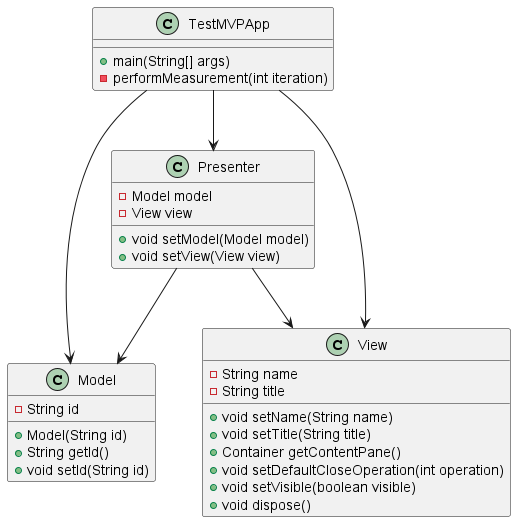
\includegraphics[width=0.5\textwidth]{../uml/mvp_diagram.png}
		\caption{Class Diagram Arsitektur MVP}
		\label{fig:class_mvp}
	\end{figure}
	
	\paragraph{Sequence Diagram}
	Diagram urutan MVP menunjukkan bahwa proses dimulai ketika pengguna mengubah nilai inputSpinner di View. View mendeteksi perubahan dan mengirimkan acara ke Presenter. Presenter kemudian memperoleh nilai terbaru dari inputSpinner dan mengubah Model, yang kemudian memperbarui data. Presenter memperoleh nilai baru dari Model dan mengubah outputSpinner di View, yang menampilkan nilai baru tersebut. MVP mengelola data dan interaksi pengguna secara langsung antara Model dan View melalui Presenter.
	
	\begin{figure}[h]
		\centering
		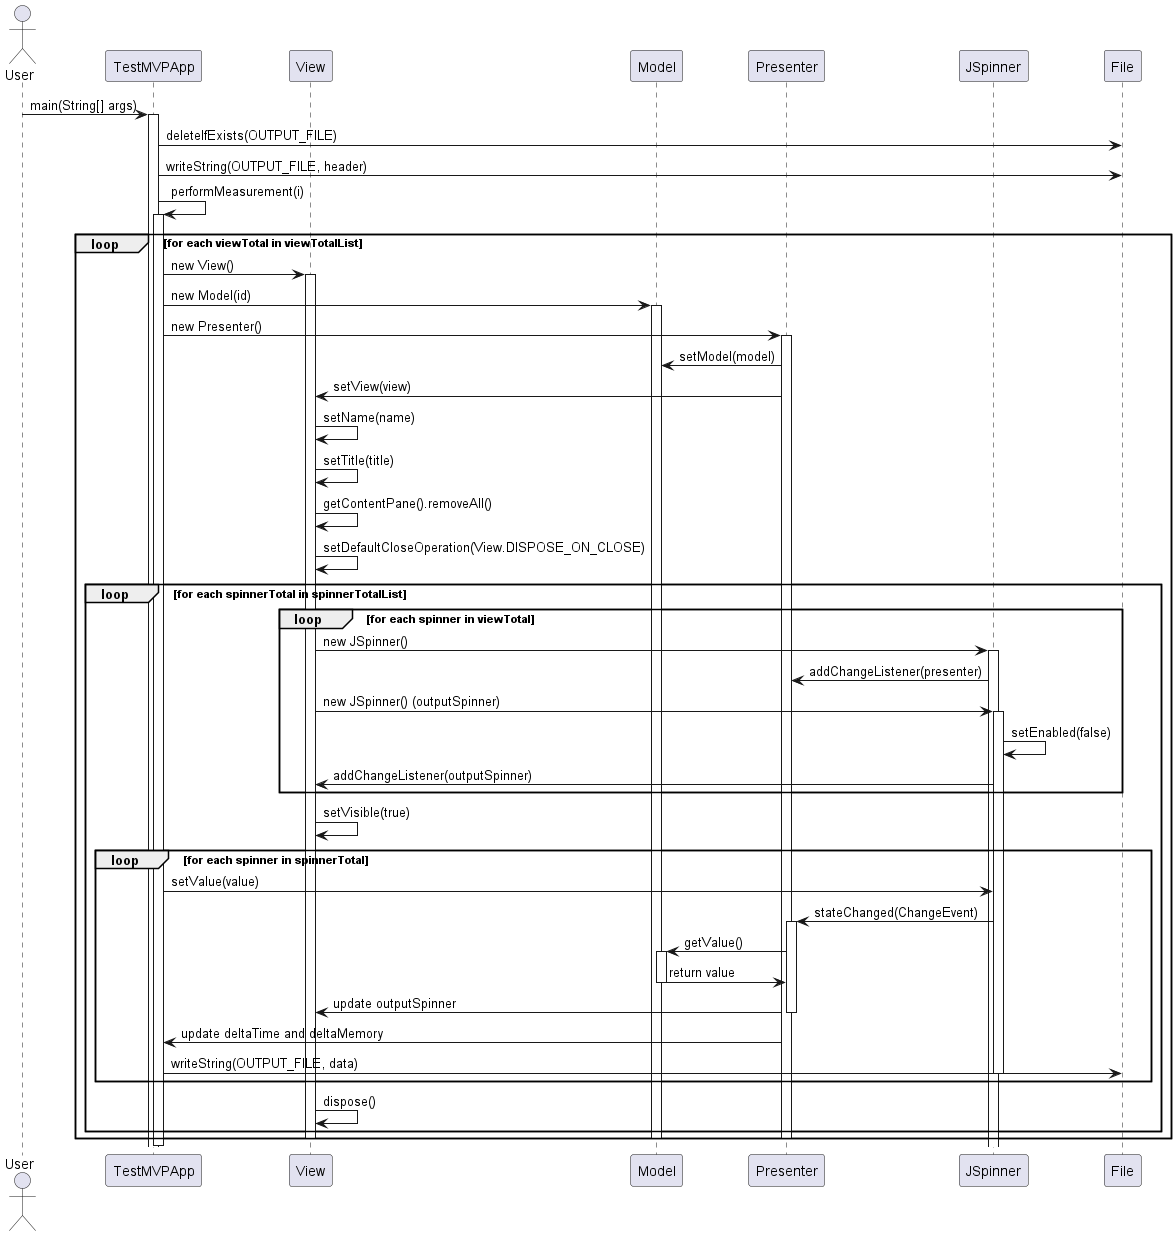
\includegraphics[width=0.5\textwidth]{../uml/mvp_sequence.png}
		\caption{Sequence Diagram Arsitektur MVP}
		\label{fig:sequence_mvp}
	\end{figure}
	
	\subsubsection{Pola Arsitektur MVVM}
	\paragraph{Class Diagram}
	Diagram kelas Unified Modeling Language (UML) yang disediakan menunjukkan pola arsitektur MVVM (Model-View-ViewModel), yang banyak digunakan dalam pengembangan perangkat lunak, terutama dalam sistem dengan antarmuka pengguna grafis (GUI). Seperti pada gambar \ref{fig:class_mvvm}, diagram ini memiliki tiga komponen utama: Model, View, dan ViewModel \cite{ri2023}.
	
	Kelas model mewakili data dan logika bisnis aplikasi. Ini termasuk properti data yang menyimpan data aplikasi, serta metode untuk mengambil dan memodifikasi data tersebut. Model bertanggung jawab untuk memelihara status data dan aturan bisnis aplikasi.
	
	Antarmuka IView mewakili kontrak tampilan aplikasi. Ini mendefinisikan fungsi updateView(data: String), yang harus digunakan oleh tampilan untuk memperbarui tampilan mereka sebagai respons terhadap perubahan dalam data.
	
	Kelas View mengimplementasikan antarmuka IView dan menyediakan antarmuka pengguna (UI) aplikasi. Ini memiliki fungsi updateView(data: String) yang memperbarui tampilan berdasarkan perubahan dalam data. Ini juga dapat memiliki metode untuk menangani interaksi pengguna, seperti userAction().
	
	Kelas ViewModel berfungsi sebagai perantara antara Model dan View. Ini mencakup referensi ke Model dan View (melalui atribut pribadi -model: Model dan -view: IView). Fungsi utama ViewModel adalah mengirim data dari Model ke View dan mengubah Model sebagai respons terhadap interaksi pengguna di View. Ini menawarkan metode seperti onDataChanged(data: String) yang memberi tahu View tentang perubahan data dan requestData(), yang memulai pengambilan data dari model.
	
	ViewModel ini tergantung pada baik Model maupun View, karena ia memanipulasi Model dan memperbarui View sebagai respons terhadap perubahan Model. View bergantung pada ViewModel untuk menangani perubahan data dan interaksi pengguna. ViewModel berkomunikasi dengan Model untuk mengambil atau memperbarui informasi. Secara keseluruhan, paradigma MVVM membedakan antara manajemen data (Model), antarmuka pengguna (View), dan logika perantara (ViewModel), memungkinkan modularitas, uji coba, dan keberlanjutan dalam program perangkat lunak.
	
	\begin{figure}[h]
		\centering
		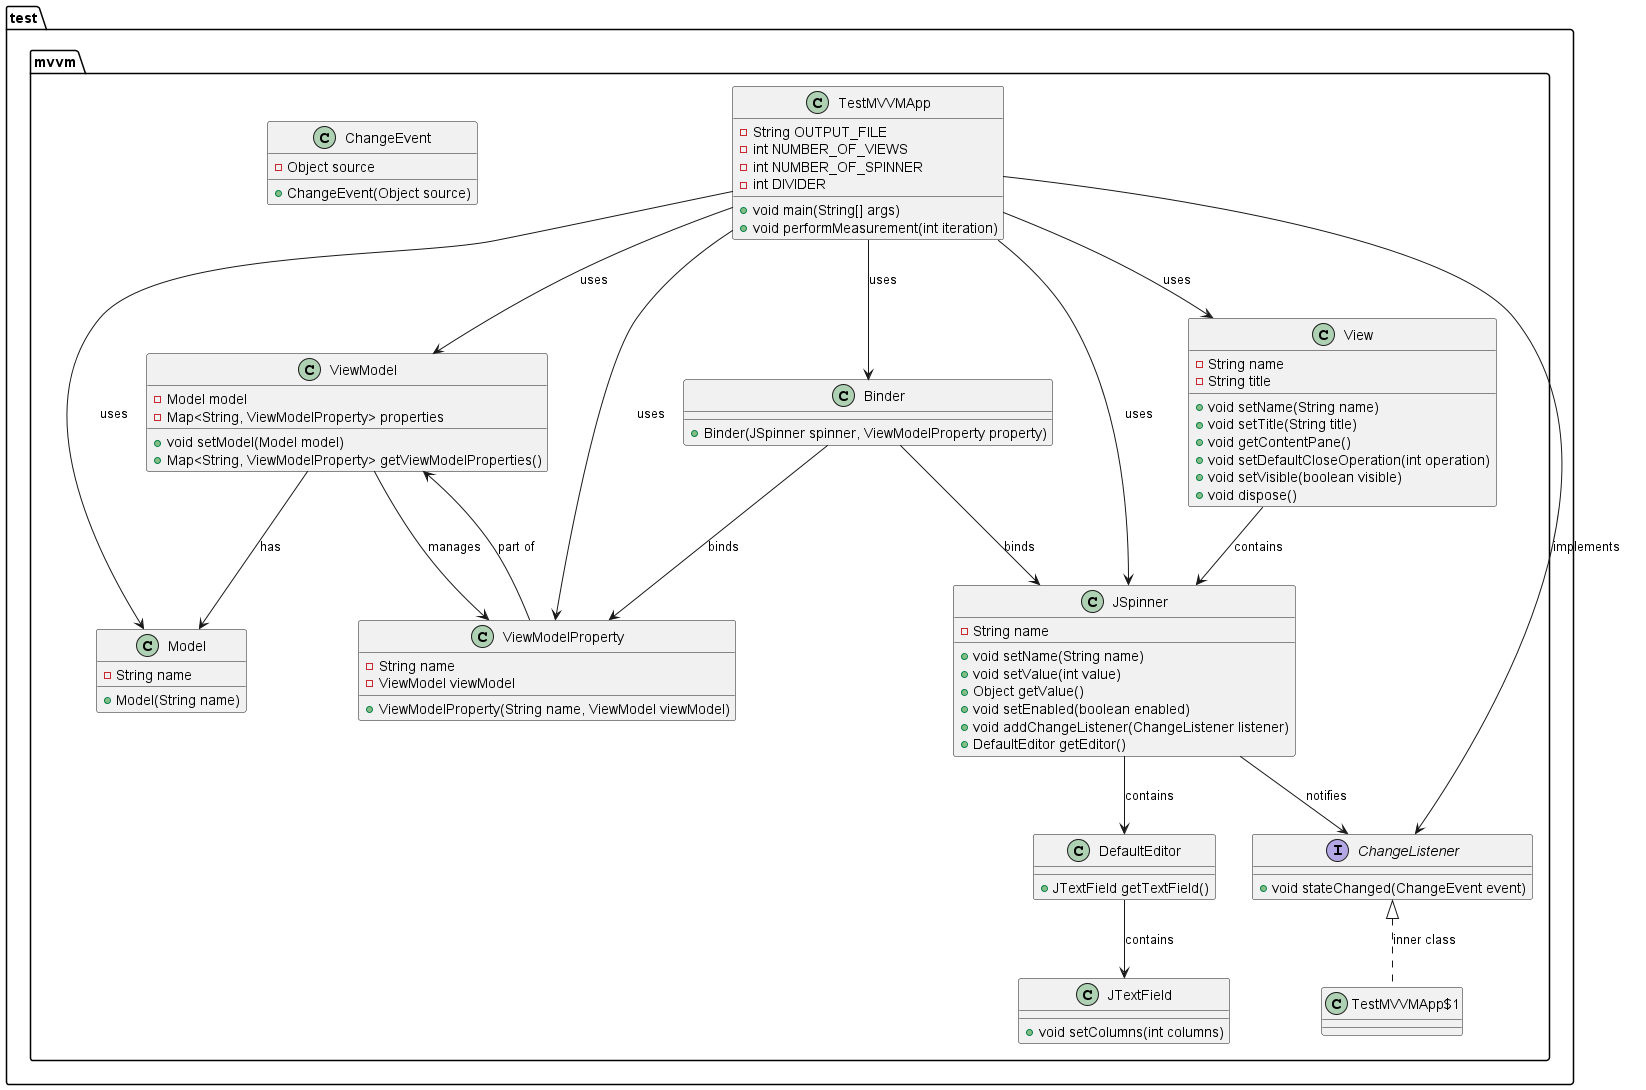
\includegraphics[width=0.5\textwidth]{../uml/mvvm_class.png}
		\caption{Class Diagram Arsitektur MVVM}
		\label{fig:class_mvvm}
	\end{figure}
	
	\paragraph{Sequence Diagram}
	Diagram urutan MVVM menunjukkan bahwa proses dimulai ketika pengguna mengubah nilai pada inputSpinner di View. Binder mengenali perubahan tersebut dan mengubah ViewModelProperty yang sesuai. ViewModelProperty mengubah data di ViewModel, yang kemudian memperbarui Model dengan nilai baru. Model mengubah datanya, dan ViewModel mengenali perubahan tersebut dan memperbarui ViewModelProperty yang sesuai. Binder mendeteksi perubahan pada ViewModelProperty dan mengubah outputSpinner di View, menampilkan nilai baru tersebut. MVVM mengelola pengikatan data dengan cara yang lebih sistematis, mengisolasi fungsi aplikasi dari komponen UI.
	
	\vspace{5 cm} 
	
	\begin{figure}[h]
		\centering
		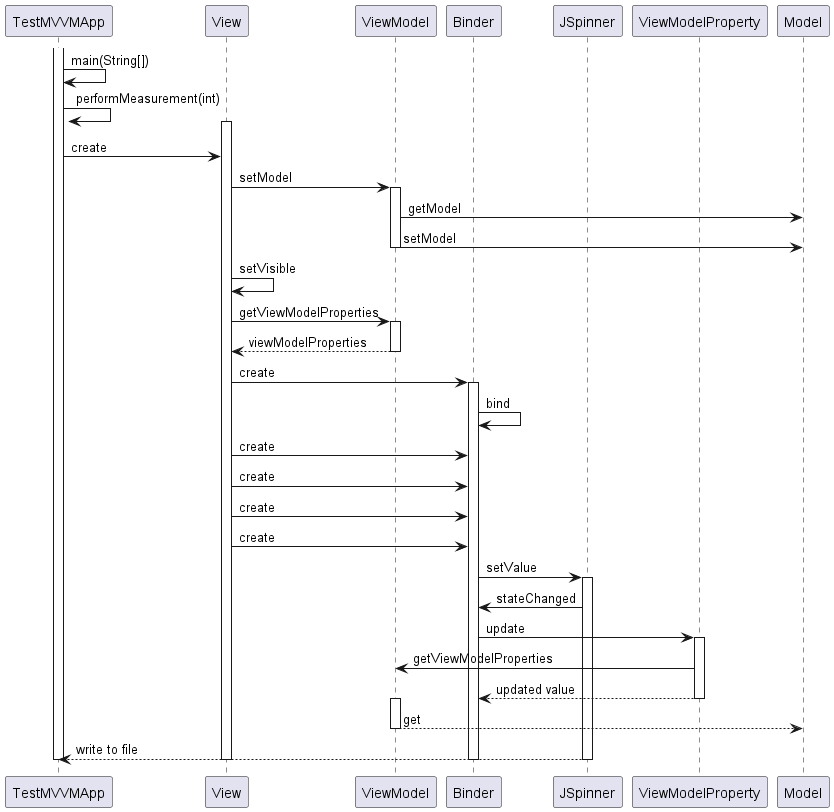
\includegraphics[width=0.5\textwidth]{../uml/mvvm_sequence.png}
		\caption{Sequence Diagram Arsitektur MVVM}
		\label{fig:sequence_mvvm}
	\end{figure}
	
	\subsection{Implementasi}
	\subsubsection{Pola Arsitektur MVP}
	Dalam arsitektur MVP, \textit{Model}, \textit{View}, dan \textit{Presenter} bekerja bersama untuk menciptakan struktur aplikasi yang terorganisir dengan baik. Kelas \textit{Model} bertanggung jawab dalam mengelola data aplikasi, memiliki atribut nama dan peta pasangan kunci-nilai, serta metode untuk mengatur dan mendapatkan nilai-nilai ini. Kelas \textit{View} bertugas dalam menangani antarmuka pengguna, menggunakan komponen Swing seperti 'JFrame' dan 'JSpinner'. Kelas \textit{View} juga mengatur jendela dan spinner serta memungkinkan \textit{Presenter} untuk mendaftar sebagai pendengar perubahan pada spinner. Kelas \textit{Presenter} berfungsi sebagai perantara antara \textit{Model} dan \textit{View}. Ketika pengguna mengubah nilai spinner, metode \textit{'stateChanged'} dalam \textit{Presenter} dipicu, yang memperbarui \textit{model} dan mencerminkan perubahan tersebut di \textit{View} dengan memperbarui spinner output yang sesuai.
	
	\subsubsection{Pola Arsitektur MVVM}
	Implementasi dari arsitektur MVVM dilakukan dengan aplikasi Java Swing. Pada pola MVVM, adanya 6 kelas yang dibuat yaitu, \textit{Binder}, \textit{Model}, \textit{View}, \textit{ViewModel}, \textit{ViewModelProperty}, dan \textit{ViewModelPropertyChangeEvent}.
	
	Kelas \textit{Binder} bertanggung jawab untuk mengikat properti-properti antara JSpinner dan \textit{ViewModelProperty}. Ketika nilai JSpinner berubah, \textit{Binder} akan mengatur nilai yang sesuai pada \textit{ViewModelProperty}, dan sebaliknya.
	
	Kelas \textit{Model} merepresentasikan data dan logika bisnis aplikasi. Dalam implementasi, kelas \textit{Model} memiliki sebuah nama dan kumpulan nilai-nilai yang dikaitkan dengan kunci tertentu.
	
	Kelas \textit{View} mewakili tampilan aplikasi. Di dalamnya terdapat JSpinner yang ditampilkan pada pengguna. Kelas \textit{Binder} digunakan untuk mengaitkan JSpinner dengan properti-properti \textit{ViewModel}.
	
	Kelas \textit{ViewModel} bertanggungjawab untuk mengelola data yang ditampilkan di View. Dalam implementasi ini, \textit{ViewModel} memiliki referensi ke objek \textit{Model} dan peta properti-properti yang terkait dengan JSpinner.
	
	Kelas \textit{ViewModelProperty} merepresentasikan properti di dalam \textit{ViewModel}. Properti ini memiliki nama, nilai, dan \textit{listener} perubahan nilai.
	
	\textit{ViewModelPropertyChangeEvent} merupakan \textit{interface} untuk mendefinisikan sebuah metode yang akan dipanggil ketika nilai properti berubah.
	
	\subsection{Pengujian}
	\subsubsection{Pola Arsitektur MVP}
	Setelah semua setup diimplementasikan dengan benar, maka kelas TestMVPApp.java dipanggil untuk melakukan pengujian dengan membuat beberapa \textit{view} dan mengukur kinerja. Kelas ini mengatur lingkungan uji, menyimpan semua data pengujian data dalam file 'data\_mvp.csv', dan melakukan pengukuran kinerja. Kelas ini melakukan iterasi sebanyak 12 kali melalui berbagai konfigurasi \textit{total view} dan spinner (1, 25, 50, 75, 100). Untuk setiap kombinasi, kelas ini menginisialisasi \textit{view} baru dengan \textit{Model} dan \textit{Presenter} yang terkait, mengatur input dan output spinner, dan mencatat waktu mulai saat nilai spinner input diubah. Hasilnya, termasuk nomor iterasi, \textit{total view}, nomor \textit{view}, total spinner, nomor spinner, waktu pemrosesan, dan penggunaan memori, ditulis ke 'data\_mvp.csv'. Pendekatan sistematis ini memungkinkan analisis kinerja yang mendetail dari arsitektur MVP dalam menangani beberapa \textit{view} dan interaksi pengguna secara efisien.
	
	\subsubsection{Pola Arsitektur MVVM}
	TestMVVMApp berfungsi untuk menguji kinerja arsitektur MVVM yang diimplementasikan dalam aplikasi Java Swing. Pengujian dimulai dengan membaut file baru saat pengujian berlangsung. Setiap kali aplikasi dijalankan, header untuk file CSV output juga ditampilkan di konsol untuk memastikan bahwa data yang tercatat sesuai. Kemudian, metode 'performMeasurement' melakukan pengukuran kinerja dengan menghasilkan konfigurasi berbeda untuk jumlah \textit{views} dan spinner berdasarkan nilai \textit{'divider'}. Setelah itu, untuk setiap konfigurasi \textit{view} dan spinner, aplikasi secara dinamis membuat \textit{view} dan mengaitkannya dengan spinner, \textit{model}, dan \textit{viewmodel}. Selanjutnya, \textit{binding} antara spinner input-output dan \textit{viewmodel} dilakukan dengan menggunakan kelas 'Binder'. \textit{Listener} perubahan ditempatkan pada spinner keluaran untuk mengukut metriks kinerja seperti waktu dan penggunaan memori. Setelah semua pengukuran selesai untuk satu konfigurasi, \textit{view} akan dihapus untuk membersihkan sumber daya. Hasil pengukuran, termasuk iterasi, \textit{total views}, nomor \textit{views}, total spinner, nomor spinner, waktu, dan penggunaan memori direkan dalam file 'data\_mvvm.csv' untuk analisis lebih lanjut. 
	
	\section{Hasil dan Pembahasan}
	Setelah pengujian dilakukan, data yang didapatkan, digunakan untuk menghasilkan 4 grafik dengan menggunakan python. Grafik-grafik berupa perbandingan spin atau views terhadap memori atau waktu.
	
	\subsection{Total Spin to Total Memory}
	Berdasarkan gambar \ref{fig:total_spin_to_total_memory},  pola arsitektur MVP memiliki rata-rata penggunaan memori yang meningkat dari 63,348,572 menjadi 188,011,806, seiring spin total meningkat. Rentang antar kuartil juga menunjukkan variasi penggunaan memori seiring dengan peningkatan spin total.
	
	Pola arsitektur MVVM juga memiliki rata-rata penggunaan memori yang meningkat dari 67,522,209 menjadi 188,434,529 dengan meningkatnya spin total. Rentang antar kuartil pada MVVM juga memiliki tren yang serupa dengan MVP.
	
	Secara keseluruhan, kedua arsitektur menunjukkan peningkatan penggunaan memori yang signifikan dengan meningkatnya spin total. Namun, MVVM sedikit lebih efisien dalam penggunaan memori pada setiap tingkat spin total dibandingkan dengan MVP. 
	
	\begin{figure}[h]
		\centering
		\includegraphics[width=0.5\textwidth]{../mvc-mvp-mvvm-main/mvc-mvp-mvvm/plot_spin_total_memory.pdf}
		\caption{Perbandingan \textit{Total Spin to Total Memory}}
		\label{fig:total_spin_to_total_memory}
	\end{figure}
	
	\subsection{Total Spin to Total Time}
	Berdasarkan gambar \ref{fig:total_spin_to_total_time}, pola arsitektur MVP memiliki rata-rata waktu eksekusi yang meningkat dari 8051 menjadi 9324 dengan meningkatnya spin total dari 25 hingga 100. Rentang antar kuartil juga menunjukkan peningkatan. Hal ini menunjukkan bahwa pola MVP memiliki variasi yang lebih besar dalam waktu eksekusi saat spin total meningkat.
	
	Sedangkan pola arsitektur MVVM memiliki rata-rata waktu eksekusi menurun dari 2355 menjadi 2205 saat spin total meningkat. Rentang antar kuartil juga relatif konstan dibandingkan MVP, menunjukkan konsistensi yang lebih besar dalam waktu eksekusi.
	
	Secara keseluruhan, MVVM cenderung memiliki waktu eksekusi yang lebih cepat dan lebih konsisten dibandingkan arsitektur MVP saat spin total meningkat. Hal ini menunjukkan bahwa MVVM lebih efisien dalam menangani peningkatan beban kerja.
	
	\vspace{5cm}
	
	\begin{figure}[h]
		\centering
		\includegraphics[width=0.5\textwidth]{../mvc-mvp-mvvm-main/mvc-mvp-mvvm/plot_spin_total_time.pdf}
		\caption{Perbandingan \textit{Total Spin to Total Time}}
		\label{fig:total_spin_to_total_time}
	\end{figure}
	
	\subsection{Total View to Total Memory}
	Berdasarkan gambar \ref{fig:total_view_to_total_memory}, pola arsitektur MVP memiliki rata-rata penggunaan memori yang meningkat dari 71,648,523 menjadi 181,236,424, seiring meningkatnya total view. 
	
	Pola arsitektur MVVM juga memiliki tren yang serupa dengan MVP dengan rata-rata penggunaan memori meningkat dari 73,473,020 menjadi 185,514,464. 
	
	Walaupun kedua pola arsitektur memiliki tren yang meningkat, pola MVP lebih efisien dalam penggunaan memori dibandingkan MVVM. Hal ini berarti MVP menggunakan lebih sedikit memori untuk jumlah view yang sama.
	
	\begin{figure}[h]
		\centering
		\includegraphics[width=0.5\textwidth]{../mvc-mvp-mvvm-main/mvc-mvp-mvvm/plot_view_total_memory.pdf}
		\caption{Perbandingan \textit{Total View to Total Memory}}
		\label{fig:total_view_to_total_memory}
	\end{figure}
	
	\subsection{Total View to Total Time}
	Berdasarkan gambar \ref{fig:total_view_to_total_time}, pola arsitektur MVP memiliki rata-rata waktu eksekusi yang berpola 'U-shaped'. Rata-rata waktu eksekusi pada view total 25 hingga 75 menurun dari 9567 menjadi 8402, kemudian naik menjadi 8909 pada view total 100.
	
	Sedangkan pola arsitektur MVVM memiliki rata-rata waktu eksekusi menurun, yaitu dari 2417 menjadi 2170.
	
	Secara keseluruhan, pola MVVM menunjukkan waktu eksekusi yang lebih cepat daripada MVP untuk semua view total yang diuji.
	
	\vspace{5cm} 
	
	\begin{figure}[h]
		\centering
		\includegraphics[width=0.5\textwidth]{../mvc-mvp-mvvm-main/mvc-mvp-mvvm/plot_view_total_time.pdf}
		\caption{Perbandingan \textit{Total View to Total Time}}
		\label{fig:total_view_to_total_time}
	\end{figure}	
	
	\section{Kesimpulan}
	Pola arsitektur MVP menunjukkan peningkatan penggunaan memori seiring dengan peningkatan jumlah view maupun spinner, namun MVP lebih efisien dalam penggunaan memori dibandingkan dengan MVVM pada setiap jumlah view atau spinner.
	
	Pada waktu eksekusi, MVVM menunjukkan waktu eksekusi yang lebih konsisten dan lebih cepat dibandingkan MVP pada setiap jumalh view atau spinner.
	
	Secara keseluruhan, kedua pola arsitektur memiliki kelebihan dan kekurangan masing-masing. Pemilihan antara MVP dan MVVM harus mempertimbangkan kebutuhan spesifik aplikasi, prioritas dalam efisiensi atau waktu eksekusi, serta kompleksitas pengembangan dan pemeliharaan kode.
	
\bibliography{reference.bib}

\end{document}
